\chapter{Background \& Objectives}
\label{ch:background}

The primary goal of this project was to create a fun and interesting manner to send messages between friends, while trying to design and implement something new and ingenious.\\
\\
Location Sensitive Social Notifier, or Lo Se Sono for short, offers the opportunity to be a completely new platform to communicate messages between people and be a potential public service that allows messages to be shared within a local area.

\section{Background}   

The idea behind the project was to create a location based messaging application where users could leave tags on specific locations on a map and it be picked up by the user's friends when they pass over that location. This sounds fairly mundane but it was an idea that had not been done without the help of external devices like blue tooth tags.\\
\\
Conceptually the application is interesting as it allows people to place a message, for example outside of a shop, placing a tag saying that a product within the shop is heavily discounted. Another example could be if a person was participating within a marathon and the organisers could add tags to specific points throughout the route to indicate how far a participant has completed. These messages could include useful information indicating that there is water nearby, or other interesting facts. More interestingly, friends could use it within their groups to indicate where users are meeting and sharing useful facts among their friend groups. Overall this is a fun concept that could be used for multiple different situations and we are unlikely to know all of the application's uses until it enters a production like environment where there are real users trying new things.\\
\\
The concept for the application could be very lucrative to advertisers as they could use it to advertise products that are available nearby to the current user location. This advertising could be used as a source of revenue for the application and putting up sponsored advertisements should help with the overall running and growth of the product as a whole. This could also mean that the product could be used for exhibitors, museums or galleries to attract passers-by into a building by showing them a notification about the interesting things they will discover inside.\\
\\
The concept takes hints from other applications and products to create a somewhat soci≈al media type style to its implementation, taking features from Facebook, Snapchat and Imgur, just to name a few. Strong UI cues are taken from Snapchat, with the commenting and voting system closely inspired by Imgur.

\subsection{Origin}
\label{sec:origin}

The origin of Lo Se Sono stems back to a sleepless night where the idea first occurred for a GPS-based application that would buzz in user's pockets when they were walking close to their friends to notify them to the fact that there was one of their friends nearby. This flowed into 'what if a user could leave tags/messages in a given location and their friends were notified of this tag/message that had been left?', thinking this would be a very useful idea for a group of friends to remind another member to collect a specific item.\\
\\
The idea was left for 6-7 months before thoughts of dissertations surfaced and it seemed this would be a well rounded and interesting project to implement. There were slight changes made to the concept throughout the early stages, as it was initially suggested to develop the idea with the use of 3rd party blue-tooth dongles to give a much more accurate fix on location, but it would mean that not everyone with a smart phone could use the application. The idea of having extra hardware to make the application useful, would limit the application's audience and make it difficult for the application to gain critical mass. However, relying on just GPS location sensing does mean the accuracy of the application is limited to a maximum radius of 15 meters away from the object, in most normal environments.

\subsection{Name}

The idea for the name originated while on a boring train journey to a job interview with IBM. Anyway, it was decided the project needed an interesting name and the original project title of 'Geo Location Social Messaging/Tagging Application' was not particularly snappy, so something cool and catchy was needed. The list in figure \ref{fig:list_of_names} contains the initial list of names that were considered. 

\begin{figure}[H]
\begin{itemize}
\item Geo Poke
\item Local Tagg
\item Tag Friend
\item WhatDown
\item WhatDrop
\item MessageSpot
\item TagSpot
\item WhatSpot
\item Location Sensitive Social Notifier (Lo Se Sono)
\item Geo Social Notifier
\end{itemize}
\caption{The list of possible names for the application}
\label{fig:list_of_names}
\end{figure}

\noindent
After a bit of deliberation between Geo Social Notifier and Location Sensitive Social Notifier, and trying to shorten them into something that can be used on the application name, it was felt that 'Location Sensitive Social Notifier' which shortened nicely to 'Lo Se Sono', seemed to roll nicely off the tongue. The next step was to see if the name had already been taken, and on putting the name into Google I had a nice surprise as it showed that 'Lo Se Sono' written in Italian had the translation of 'If you are' which was a cool coincidence. This fact is shown in figure \ref{fig:google_translate}.

\begin{figure}[H]
    \centering
    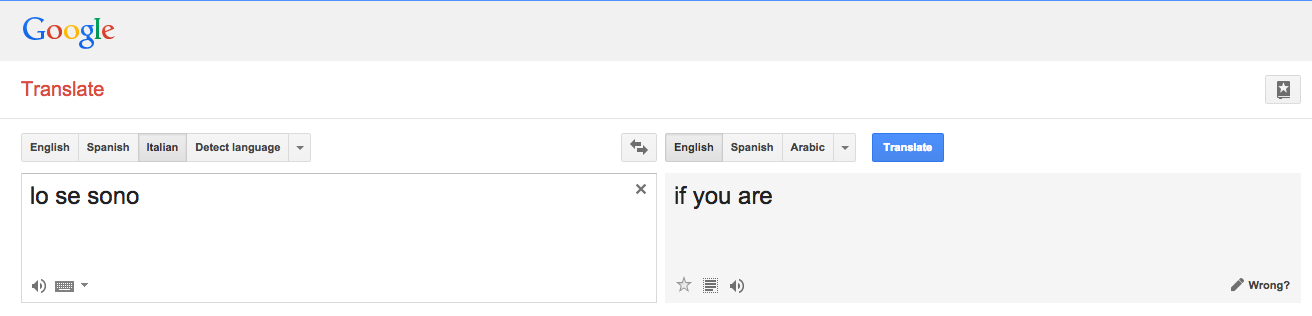
\includegraphics[width=\textwidth]{translate}
    \caption{Coincidence of the name}
    \label{fig:google_translate}
\end{figure} 

\subsection{Research}

Researching the project consisted of finding out if the idea had been implemented before. There were a few similar ideas but nothing that did it well or had major design differences. One of the similar products was named Message Drop \cite{dmt:dropmessageteam:2015:online} and was an Apple iOS exclusive. There were a few other projects that had been around in the past, but seemed to have died off or evolved into other projects.\\
\\
Once the market research was completed, attention turned to the different technologies that would have to underpin the application; most specifically GPS and which mobile operating system to code the application. The two main contenders for the latter were Android and Phonegapp, and in depth coverage of each platform can be found in Chapter \ref{ch:design} section \ref{sec:android_choice_of_tech}. Researching GPS was key to the application's success and factors that needed to be assessed included its overall accuracy, which some indicate can be between 2-40 meters \cite{DevdattaTengshe:gpsacuracy:2012:online}, depending on conditions. It became clear throughout the project that this is a much bigger problem than first thought and it is clear that GPS struggles to get a fix in anything but near perfect environments.\\
\\
Extensive research was also undertaken to look into the best ways to design Google Android applications, with a fair bit of studying of Google's own material design guides to ensure the application had a uniform look and would fit in with the Android ecosystem.\\
\\
There was considerable time taken to decide what languages \& frameworks to use for the project, weighing up the correct framework to provide the RESTful interfaces for the application. In depth explanation of the rationale behind each choice of framework can be found in Chapter \ref{ch:design}.

\subsection{Analysis}

The analysis of the problem started by thinking over the various stages of the idea. For example, posting a message, receiving a message and receiving a notification. These were then broken into the individual UI screens that would allow the user to interact with and carry out the actions within the application. Once the major UI work and a semi-sensible idea was created for that action, the thoughts turned to how to link up the screen activity to the data that would be stored that would enable the application to work.\\
\\
As the development of the application took an agile style to its methodology, each part of the application evolved incrementally. So the parts research and design of the parts grew organically to connect between the UI and the database design, which were done at the very beginning of the project. Mocking up the UI and designing the database were the main way to break the project up into its functional sections.\\
\\
More thought was given to the choice of frameworks and languages to use at the beginning, with research into which were the best platforms to use.\\
\\
All the points to do with the functional requirements and the choice of frameworks are contained within chapter \ref{ch:design}.

\section{Process}
\label{sec:methodology}

The process used for the project was a mixture of a few different agile development processes. These processes are used to organise and manage projects and they promote adaptivity and continuous improvement within the code to ensure that a well rounded product gets developed and that in a business environment that the customer needs are met.\\
\\
Even though this is an agile style of development, due to the developer and writer of this project being the customer it is fairly hard to take on all of the concepts that are encouraged by agile, as there is no migratory gap between the customer and developer. So the coping strategies implemented in the methodologies are not needed. The methodology that is used for the project takes the best bits from a couple of different methodologies and is formed together to manage the project in a specific way that should lead to a fully fledged and functional project.

\subsection{Agile}

A few points from the agile manifesto made it into the process used for the application. Rapid prototyping and regular code releases played a key part to the development of the application when the application had released a point where it could start to be used by members of the public. The first releases were made with rapid bug fixes and new features added to keep the test group interested. This led ultimately to some of the design being changed and modified throughout the deployment of the application, which is another point that agile copes with well, changing requirements throughout the development of the project; if something was not right then it was changed.\\
\\
The use of a self-organising and organic development process helped with the design and aimed to keep the development as simple as possible to minimise the choke points and to try and keep a well designed bit of software. The organic development also led to the project moving at a steady and dependable rate. Even if there was not progress made on the software itself then there would be work and activity in other areas running at a similar rate.

\subsection{Feature Driven Development}

A lot of the core concepts of Feature Driven Development (FDD) have been used with the implementation of this project. The core one is design and build by feature. The project was initially broken down into its functional areas, then the design was created and implemented to cover that functional area of the application. These steps were taken for each part of the development.\\
\\
The initial list of functional requirements that was made at the start of the project really helped break the application into manageable sections that then could be worked on to build up and create a fully working and functional application.

\subsection{eXtream Programming}

eXtream Programming (XP) is a methodology that lends itself to incremental design and development of a project. Some parts of the methodology were used most inclusively, YAGNI (You aren't going to need it), so keeping the design as simple as possible and not implementing the feature until absolutely sure that it is needed, to help keep the code base uncluttered. The use of strong unit testing was an aim as well, but due to how things are implemented in Android this has been very difficult to do, so only the backend has been unit tested to ensure it works correctly. XP allows the developer to have the courage to admit they got the design wrong and change it to suite their needs better.